\documentclass{standalone}
\usepackage{tikz}
\usetikzlibrary{patterns, positioning}

\begin{document}
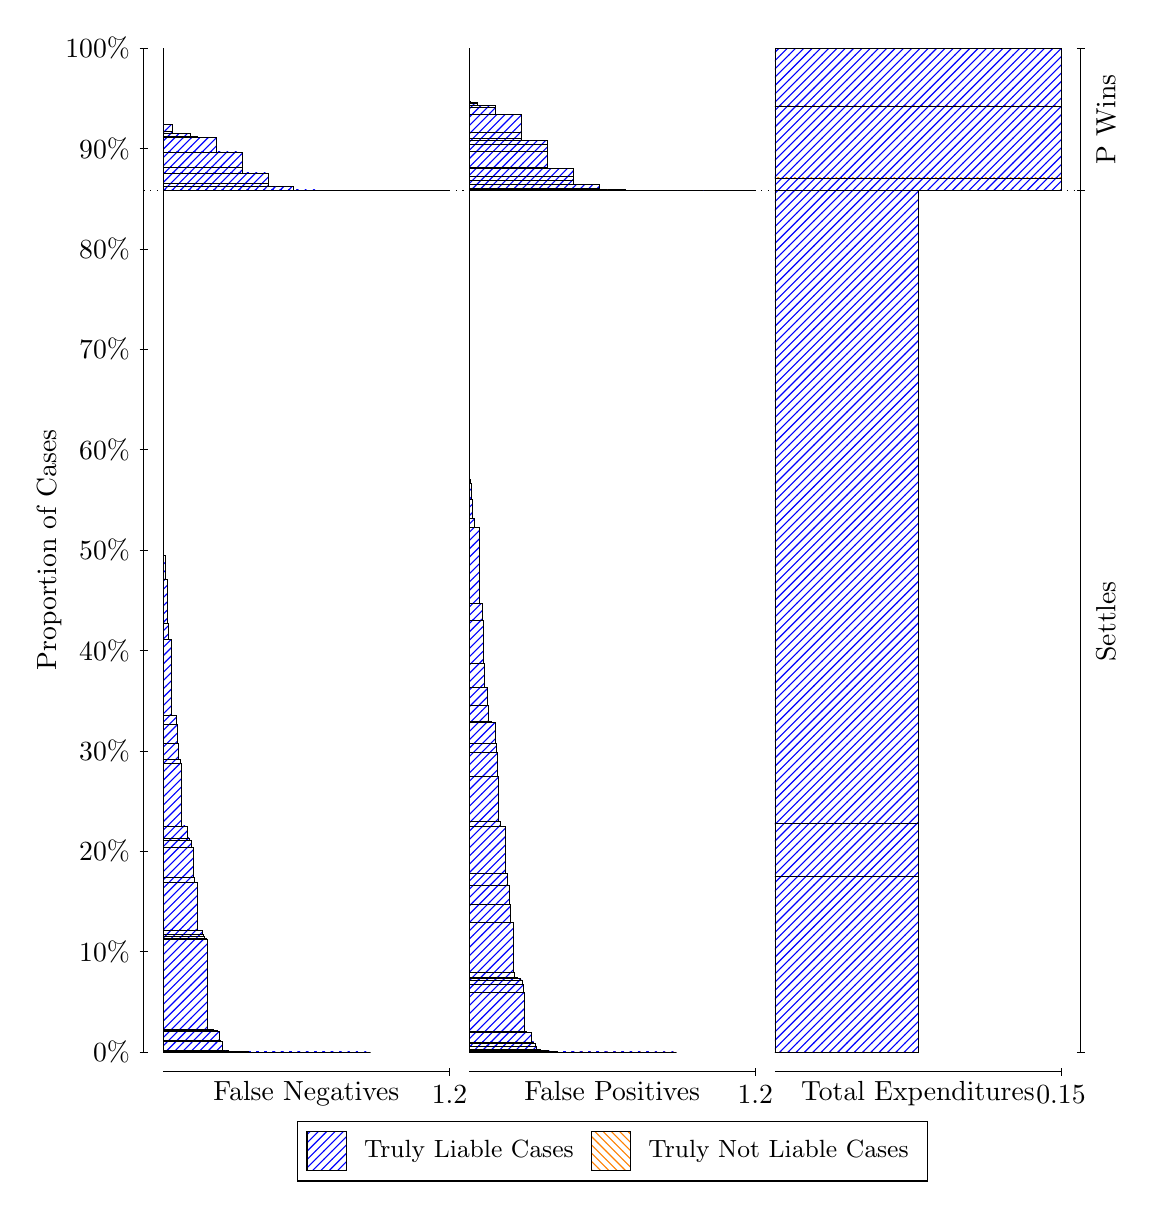
\begin{tikzpicture}
\draw[black, very thin] (1.5,1.75) -- (1.5,14.5);
\node[rotate=90, anchor=center] at (0.3, 8.125) {Proportion of Cases};
\draw[black, very thin] (1.45,1.75) -- (1.55,1.75);
\node[anchor=east] at (1.45, 1.75) {0\%};
\draw[black, very thin] (1.45,3.025) -- (1.55,3.025);
\node[anchor=east] at (1.45, 3.025) {10\%};
\draw[black, very thin] (1.45,4.3) -- (1.55,4.3);
\node[anchor=east] at (1.45, 4.3) {20\%};
\draw[black, very thin] (1.45,5.575) -- (1.55,5.575);
\node[anchor=east] at (1.45, 5.575) {30\%};
\draw[black, very thin] (1.45,6.85) -- (1.55,6.85);
\node[anchor=east] at (1.45, 6.85) {40\%};
\draw[black, very thin] (1.45,8.125) -- (1.55,8.125);
\node[anchor=east] at (1.45, 8.125) {50\%};
\draw[black, very thin] (1.45,9.4) -- (1.55,9.4);
\node[anchor=east] at (1.45, 9.4) {60\%};
\draw[black, very thin] (1.45,10.675) -- (1.55,10.675);
\node[anchor=east] at (1.45, 10.675) {70\%};
\draw[black, very thin] (1.45,11.95) -- (1.55,11.95);
\node[anchor=east] at (1.45, 11.95) {80\%};
\draw[black, very thin] (1.45,13.225) -- (1.55,13.225);
\node[anchor=east] at (1.45, 13.225) {90\%};
\draw[black, very thin] (1.45,14.5) -- (1.55,14.5);
\node[anchor=east] at (1.45, 14.5) {100\%};

\draw[black, very thin] (13.4,1.75) -- (13.4,14.5);
\draw[black, very thin] (13.35,1.75) -- (13.45,1.75);
\node[anchor=west] at (13.35, 1.75) {};
\draw[black, very thin] (13.35,12.688) -- (13.45,12.688);
\node[anchor=west] at (13.35, 12.688) {};
\draw[black, very thin] (13.35,14.5) -- (13.45,14.5);
\node[anchor=west] at (13.35, 14.5) {};

\draw[black, very thin, pattern color=blue, pattern=north east lines] (1.75,1.75) rectangle (4.3823,1.75);
\draw[black, very thin, pattern color=blue, pattern=north east lines] (1.75,1.75) rectangle (4.234,1.75);
\draw[black, very thin, pattern color=blue, pattern=north east lines] (1.75,1.75) rectangle (4.0857,1.75);
\draw[black, very thin, pattern color=blue, pattern=north east lines] (1.75,1.75) rectangle (4.0528,1.75);
\draw[black, very thin, pattern color=blue, pattern=north east lines] (1.75,1.75) rectangle (3.9374,1.75);
\draw[black, very thin, pattern color=blue, pattern=north east lines] (1.75,1.75) rectangle (3.9045,1.75);
\draw[black, very thin, pattern color=blue, pattern=north east lines] (1.75,1.75) rectangle (3.7891,1.75);
\draw[black, very thin, pattern color=blue, pattern=north east lines] (1.75,1.75) rectangle (3.7562,1.75);
\draw[black, very thin, pattern color=blue, pattern=north east lines] (1.75,1.75) rectangle (3.7232,1.75);
\draw[black, very thin, pattern color=blue, pattern=north east lines] (1.75,1.75) rectangle (3.6079,1.75);
\draw[black, very thin, pattern color=blue, pattern=north east lines] (1.75,1.75) rectangle (3.5749,1.75);
\draw[black, very thin, pattern color=blue, pattern=north east lines] (1.75,1.75) rectangle (3.4925,1.75);
\draw[black, very thin, pattern color=blue, pattern=north east lines] (1.75,1.75) rectangle (3.4596,1.75);
\draw[black, very thin, pattern color=blue, pattern=north east lines] (1.75,1.75) rectangle (3.4266,1.75);
\draw[black, very thin, pattern color=blue, pattern=north east lines] (1.75,1.75) rectangle (3.3937,1.75);
\draw[black, very thin, pattern color=blue, pattern=north east lines] (1.75,1.75) rectangle (3.3442,1.75);
\draw[black, very thin, pattern color=blue, pattern=north east lines] (1.75,1.75) rectangle (3.2783,1.75);
\draw[black, very thin, pattern color=blue, pattern=north east lines] (1.75,1.75) rectangle (3.2454,1.75);
\draw[black, very thin, pattern color=blue, pattern=north east lines] (1.75,1.75) rectangle (3.1959,1.75);
\draw[black, very thin, pattern color=blue, pattern=north east lines] (1.75,1.75) rectangle (3.163,1.7501);
\draw[black, very thin, pattern color=blue, pattern=north east lines] (1.75,1.7501) rectangle (3.13,1.7501);
\draw[black, very thin, pattern color=blue, pattern=north east lines] (1.75,1.7501) rectangle (3.0971,1.7501);
\draw[black, very thin, pattern color=blue, pattern=north east lines] (1.75,1.7501) rectangle (3.0641,1.7501);
\draw[black, very thin, pattern color=blue, pattern=north east lines] (1.75,1.7501) rectangle (3.0476,1.7501);
\draw[black, very thin, pattern color=blue, pattern=north east lines] (1.75,1.7501) rectangle (3.0147,1.7501);
\draw[black, very thin, pattern color=blue, pattern=north east lines] (1.75,1.7501) rectangle (2.9488,1.7501);
\draw[black, very thin, pattern color=blue, pattern=north east lines] (1.75,1.7501) rectangle (2.9158,1.7501);
\draw[black, very thin, pattern color=blue, pattern=north east lines] (1.75,1.7501) rectangle (2.8993,1.7505);
\draw[black, very thin, pattern color=blue, pattern=north east lines] (1.75,1.7505) rectangle (2.8664,1.7505);
\draw[black, very thin, pattern color=blue, pattern=north east lines] (1.75,1.7505) rectangle (2.8334,1.7562);
\draw[black, very thin, pattern color=blue, pattern=north east lines] (1.75,1.7562) rectangle (2.8005,1.7563);
\draw[black, very thin, pattern color=blue, pattern=north east lines] (1.75,1.7563) rectangle (2.7675,1.7564);
\draw[black, very thin, pattern color=blue, pattern=north east lines] (1.75,1.7564) rectangle (2.7345,1.7564);
\draw[black, very thin, pattern color=blue, pattern=north east lines] (1.75,1.7564) rectangle (2.7181,1.7569);
\draw[black, very thin, pattern color=blue, pattern=north east lines] (1.75,1.7569) rectangle (2.6851,1.7569);
\draw[black, very thin, pattern color=blue, pattern=north east lines] (1.75,1.7569) rectangle (2.6192,1.7571);
\draw[black, very thin, pattern color=blue, pattern=north east lines] (1.75,1.7571) rectangle (2.6027,1.7582);
\draw[black, very thin, pattern color=blue, pattern=north east lines] (1.75,1.7582) rectangle (2.5862,1.7587);
\draw[black, very thin, pattern color=blue, pattern=north east lines] (1.75,1.7587) rectangle (2.5698,1.7666);
\draw[black, very thin, pattern color=blue, pattern=north east lines] (1.75,1.7666) rectangle (2.5368,1.7666);
\draw[black, very thin, pattern color=blue, pattern=north east lines] (1.75,1.7666) rectangle (2.5039,1.8879);
\draw[black, very thin, pattern color=blue, pattern=north east lines] (1.75,1.8879) rectangle (2.4709,1.8931);
\draw[black, very thin, pattern color=blue, pattern=north east lines] (1.75,1.8931) rectangle (2.4544,2.0147);
\draw[black, very thin, pattern color=blue, pattern=north east lines] (1.75,2.0147) rectangle (2.4379,2.0199);
\draw[black, very thin, pattern color=blue, pattern=north east lines] (1.75,2.0199) rectangle (2.405,2.0204);
\draw[black, very thin, pattern color=blue, pattern=north east lines] (1.75,2.0204) rectangle (2.3885,2.0412);
\draw[black, very thin, pattern color=blue, pattern=north east lines] (1.75,2.0412) rectangle (2.3556,2.0414);
\draw[black, very thin, pattern color=blue, pattern=north east lines] (1.75,2.0414) rectangle (2.3061,3.1828);
\draw[black, very thin, pattern color=blue, pattern=north east lines] (1.75,3.1828) rectangle (2.2896,3.1897);
\draw[black, very thin, pattern color=blue, pattern=north east lines] (1.75,3.1897) rectangle (2.2732,3.2165);
\draw[black, very thin, pattern color=blue, pattern=north east lines] (1.75,3.2165) rectangle (2.2567,3.2422);
\draw[black, very thin, pattern color=blue, pattern=north east lines] (1.75,3.2422) rectangle (2.2402,3.3013);
\draw[black, very thin, pattern color=blue, pattern=north east lines] (1.75,3.3013) rectangle (2.2073,3.3014);
\draw[black, very thin, pattern color=blue, pattern=north east lines] (1.75,3.3014) rectangle (2.1743,3.9001);
\draw[black, very thin, pattern color=blue, pattern=north east lines] (1.75,3.9001) rectangle (2.1413,3.9671);
\draw[black, very thin, pattern color=blue, pattern=north east lines] (1.75,3.9671) rectangle (2.1249,4.3506);
\draw[black, very thin, pattern color=blue, pattern=north east lines] (1.75,4.3506) rectangle (2.1084,4.4438);
\draw[black, very thin, pattern color=blue, pattern=north east lines] (1.75,4.4438) rectangle (2.0754,4.4675);
\draw[black, very thin, pattern color=blue, pattern=north east lines] (1.75,4.4675) rectangle (2.059,4.618);
\draw[black, very thin, pattern color=blue, pattern=north east lines] (1.75,4.618) rectangle (2.026,4.6199);
\draw[black, very thin, pattern color=blue, pattern=north east lines] (1.75,4.6199) rectangle (1.9766,5.4123);
\draw[black, very thin, pattern color=blue, pattern=north east lines] (1.75,5.4123) rectangle (1.9601,5.4705);
\draw[black, very thin, pattern color=blue, pattern=north east lines] (1.75,5.4705) rectangle (1.9436,5.6654);
\draw[black, very thin, pattern color=blue, pattern=north east lines] (1.75,5.6654) rectangle (1.9271,5.9092);
\draw[black, very thin, pattern color=blue, pattern=north east lines] (1.75,5.9092) rectangle (1.9107,6.0305);
\draw[black, very thin, pattern color=blue, pattern=north east lines] (1.75,6.0305) rectangle (1.8777,6.031);
\draw[black, very thin, pattern color=blue, pattern=north east lines] (1.75,6.031) rectangle (1.8447,6.9885);
\draw[black, very thin, pattern color=blue, pattern=north east lines] (1.75,6.9885) rectangle (1.8118,7.1998);
\draw[black, very thin, pattern color=blue, pattern=north east lines] (1.75,7.1998) rectangle (1.7953,7.7524);
\draw[black, very thin, pattern color=blue, pattern=north east lines] (1.75,7.7524) rectangle (1.7788,8.0612);
\draw[black, very thin, pattern color=orange, pattern=north west lines] (1.75,8.0612) rectangle (1.75,8.0612);
\draw[black, very thin, pattern color=blue, pattern=north east lines] (1.75,8.0612) rectangle (1.75,12.688);
\draw[black, very thin, pattern color=blue, pattern=north east lines] (1.75,12.688) rectangle (5.3833,12.688);
\draw[black, very thin, pattern color=blue, pattern=north east lines] (1.75,12.688) rectangle (5.0538,12.688);
\draw[black, very thin, pattern color=blue, pattern=north east lines] (1.75,12.688) rectangle (4.7242,12.688);
\draw[black, very thin, pattern color=blue, pattern=north east lines] (1.75,12.688) rectangle (4.3947,12.689);
\draw[black, very thin, pattern color=blue, pattern=north east lines] (1.75,12.689) rectangle (4.0651,12.689);
\draw[black, very thin, pattern color=blue, pattern=north east lines] (1.75,12.689) rectangle (4.0651,12.69);
\draw[black, very thin, pattern color=blue, pattern=north east lines] (1.75,12.69) rectangle (3.8344,12.69);
\draw[black, very thin, pattern color=blue, pattern=north east lines] (1.75,12.69) rectangle (3.7356,12.694);
\draw[black, very thin, pattern color=blue, pattern=north east lines] (1.75,12.694) rectangle (3.7356,12.698);
\draw[black, very thin, pattern color=blue, pattern=north east lines] (1.75,12.698) rectangle (3.5049,12.698);
\draw[black, very thin, pattern color=blue, pattern=north east lines] (1.75,12.698) rectangle (3.5049,12.698);
\draw[black, very thin, pattern color=blue, pattern=north east lines] (1.75,12.698) rectangle (3.406,12.745);
\draw[black, very thin, pattern color=blue, pattern=north east lines] (1.75,12.745) rectangle (3.406,12.747);
\draw[black, very thin, pattern color=blue, pattern=north east lines] (1.75,12.747) rectangle (3.1753,12.747);
\draw[black, very thin, pattern color=blue, pattern=north east lines] (1.75,12.747) rectangle (3.1753,12.747);
\draw[black, very thin, pattern color=blue, pattern=north east lines] (1.75,12.747) rectangle (3.1753,12.747);
\draw[black, very thin, pattern color=blue, pattern=north east lines] (1.75,12.747) rectangle (3.0765,12.777);
\draw[black, very thin, pattern color=blue, pattern=north east lines] (1.75,12.777) rectangle (3.0765,12.913);
\draw[black, very thin, pattern color=blue, pattern=north east lines] (1.75,12.913) rectangle (2.8458,12.913);
\draw[black, very thin, pattern color=blue, pattern=north east lines] (1.75,12.913) rectangle (2.8458,12.913);
\draw[black, very thin, pattern color=blue, pattern=north east lines] (1.75,12.913) rectangle (2.7469,12.991);
\draw[black, very thin, pattern color=blue, pattern=north east lines] (1.75,12.991) rectangle (2.7469,13.175);
\draw[black, very thin, pattern color=blue, pattern=north east lines] (1.75,13.175) rectangle (2.7469,13.181);
\draw[black, very thin, pattern color=blue, pattern=north east lines] (1.75,13.181) rectangle (2.5162,13.181);
\draw[black, very thin, pattern color=blue, pattern=north east lines] (1.75,13.181) rectangle (2.5162,13.181);
\draw[black, very thin, pattern color=blue, pattern=north east lines] (1.75,13.181) rectangle (2.5162,13.182);
\draw[black, very thin, pattern color=blue, pattern=north east lines] (1.75,13.182) rectangle (2.4173,13.363);
\draw[black, very thin, pattern color=blue, pattern=north east lines] (1.75,13.363) rectangle (2.1867,13.376);
\draw[black, very thin, pattern color=blue, pattern=north east lines] (1.75,13.376) rectangle (2.1867,13.376);
\draw[black, very thin, pattern color=blue, pattern=north east lines] (1.75,13.376) rectangle (2.0878,13.377);
\draw[black, very thin, pattern color=blue, pattern=north east lines] (1.75,13.377) rectangle (2.0878,13.418);
\draw[black, very thin, pattern color=blue, pattern=north east lines] (1.75,13.418) rectangle (2.0878,13.418);
\draw[black, very thin, pattern color=blue, pattern=north east lines] (1.75,13.418) rectangle (1.8571,13.441);
\draw[black, very thin, pattern color=blue, pattern=north east lines] (1.75,13.441) rectangle (1.8571,13.533);
\draw[black, very thin, pattern color=blue, pattern=north east lines] (1.75,13.533) rectangle (1.7582,13.534);
\draw[black, very thin, pattern color=blue, pattern=north east lines] (1.75,13.534) rectangle (1.7582,13.534);
\draw[black, very thin, pattern color=orange, pattern=north west lines] (1.75,13.534) rectangle (1.75,13.534);
\draw[black, very thin, pattern color=blue, pattern=north east lines] (1.75,13.534) rectangle (1.75,14.5);
\draw[black, very thin, pattern color=orange, pattern=north west lines] (5.6333,1.75) rectangle (8.2656,1.75);
\draw[black, very thin, pattern color=blue, pattern=north east lines] (5.6333,1.75) rectangle (8.2656,1.75);
\draw[black, very thin, pattern color=orange, pattern=north west lines] (5.6333,1.75) rectangle (8.1173,1.75);
\draw[black, very thin, pattern color=blue, pattern=north east lines] (5.6333,1.75) rectangle (8.1173,1.75);
\draw[black, very thin, pattern color=orange, pattern=north west lines] (5.6333,1.75) rectangle (7.969,1.75);
\draw[black, very thin, pattern color=blue, pattern=north east lines] (5.6333,1.75) rectangle (7.969,1.75);
\draw[black, very thin, pattern color=blue, pattern=north east lines] (5.6333,1.75) rectangle (7.9361,1.75);
\draw[black, very thin, pattern color=blue, pattern=north east lines] (5.6333,1.75) rectangle (7.7878,1.75);
\draw[black, very thin, pattern color=orange, pattern=north west lines] (5.6333,1.75) rectangle (7.6724,1.75);
\draw[black, very thin, pattern color=blue, pattern=north east lines] (5.6333,1.75) rectangle (7.6724,1.75);
\draw[black, very thin, pattern color=blue, pattern=north east lines] (5.6333,1.75) rectangle (7.6395,1.75);
\draw[black, very thin, pattern color=blue, pattern=north east lines] (5.6333,1.75) rectangle (7.6065,1.75);
\draw[black, very thin, pattern color=orange, pattern=north west lines] (5.6333,1.75) rectangle (7.5241,1.75);
\draw[black, very thin, pattern color=blue, pattern=north east lines] (5.6333,1.75) rectangle (7.5241,1.75);
\draw[black, very thin, pattern color=blue, pattern=north east lines] (5.6333,1.75) rectangle (7.4582,1.75);
\draw[black, very thin, pattern color=orange, pattern=north west lines] (5.6333,1.75) rectangle (7.3759,1.75);
\draw[black, very thin, pattern color=blue, pattern=north east lines] (5.6333,1.75) rectangle (7.3759,1.75);
\draw[black, very thin, pattern color=blue, pattern=north east lines] (5.6333,1.75) rectangle (7.3429,1.75);
\draw[black, very thin, pattern color=blue, pattern=north east lines] (5.6333,1.75) rectangle (7.3099,1.75);
\draw[black, very thin, pattern color=blue, pattern=north east lines] (5.6333,1.75) rectangle (7.277,1.75);
\draw[black, very thin, pattern color=orange, pattern=north west lines] (5.6333,1.75) rectangle (7.2276,1.75);
\draw[black, very thin, pattern color=blue, pattern=north east lines] (5.6333,1.75) rectangle (7.2276,1.75);
\draw[black, very thin, pattern color=blue, pattern=north east lines] (5.6333,1.75) rectangle (7.1946,1.75);
\draw[black, very thin, pattern color=blue, pattern=north east lines] (5.6333,1.75) rectangle (7.1287,1.75);
\draw[black, very thin, pattern color=orange, pattern=north west lines] (5.6333,1.75) rectangle (7.0793,1.75);
\draw[black, very thin, pattern color=blue, pattern=north east lines] (5.6333,1.75) rectangle (7.0793,1.7501);
\draw[black, very thin, pattern color=blue, pattern=north east lines] (5.6333,1.7501) rectangle (7.0463,1.7501);
\draw[black, very thin, pattern color=blue, pattern=north east lines] (5.6333,1.7501) rectangle (7.0133,1.7501);
\draw[black, very thin, pattern color=blue, pattern=north east lines] (5.6333,1.7501) rectangle (6.9804,1.7502);
\draw[black, very thin, pattern color=blue, pattern=north east lines] (5.6333,1.7502) rectangle (6.9474,1.7502);
\draw[black, very thin, pattern color=blue, pattern=north east lines] (5.6333,1.7502) rectangle (6.898,1.7502);
\draw[black, very thin, pattern color=blue, pattern=north east lines] (5.6333,1.7502) rectangle (6.865,1.7502);
\draw[black, very thin, pattern color=blue, pattern=north east lines] (5.6333,1.7502) rectangle (6.7991,1.7508);
\draw[black, very thin, pattern color=orange, pattern=north west lines] (5.6333,1.7508) rectangle (6.7827,1.7508);
\draw[black, very thin, pattern color=blue, pattern=north east lines] (5.6333,1.7508) rectangle (6.7827,1.7518);
\draw[black, very thin, pattern color=blue, pattern=north east lines] (5.6333,1.7518) rectangle (6.7497,1.7583);
\draw[black, very thin, pattern color=blue, pattern=north east lines] (5.6333,1.7583) rectangle (6.7167,1.7583);
\draw[black, very thin, pattern color=blue, pattern=north east lines] (5.6333,1.7583) rectangle (6.6838,1.7585);
\draw[black, very thin, pattern color=blue, pattern=north east lines] (5.6333,1.7585) rectangle (6.6508,1.7637);
\draw[black, very thin, pattern color=orange, pattern=north west lines] (5.6333,1.7637) rectangle (6.6344,1.7637);
\draw[black, very thin, pattern color=blue, pattern=north east lines] (5.6333,1.7637) rectangle (6.6344,1.774);
\draw[black, very thin, pattern color=blue, pattern=north east lines] (5.6333,1.774) rectangle (6.6179,1.7745);
\draw[black, very thin, pattern color=blue, pattern=north east lines] (5.6333,1.7745) rectangle (6.5684,1.7747);
\draw[black, very thin, pattern color=blue, pattern=north east lines] (5.6333,1.7747) rectangle (6.5355,1.7799);
\draw[black, very thin, pattern color=orange, pattern=north west lines] (5.6333,1.7799) rectangle (6.4861,1.7799);
\draw[black, very thin, pattern color=blue, pattern=north east lines] (5.6333,1.7799) rectangle (6.4861,1.8287);
\draw[black, very thin, pattern color=blue, pattern=north east lines] (5.6333,1.8287) rectangle (6.4696,1.8545);
\draw[black, very thin, pattern color=blue, pattern=north east lines] (5.6333,1.8545) rectangle (6.4531,1.8781);
\draw[black, very thin, pattern color=blue, pattern=north east lines] (5.6333,1.8781) rectangle (6.4201,2.0009);
\draw[black, very thin, pattern color=blue, pattern=north east lines] (5.6333,2.0009) rectangle (6.3872,2.001);
\draw[black, very thin, pattern color=blue, pattern=north east lines] (5.6333,2.001) rectangle (6.3542,2.0079);
\draw[black, very thin, pattern color=orange, pattern=north west lines] (5.6333,2.0079) rectangle (6.3378,2.0079);
\draw[black, very thin, pattern color=blue, pattern=north east lines] (5.6333,2.0079) rectangle (6.3378,2.5115);
\draw[black, very thin, pattern color=blue, pattern=north east lines] (5.6333,2.5115) rectangle (6.3213,2.6046);
\draw[black, very thin, pattern color=blue, pattern=north east lines] (5.6333,2.6046) rectangle (6.3048,2.6657);
\draw[black, very thin, pattern color=blue, pattern=north east lines] (5.6333,2.6657) rectangle (6.2883,2.6919);
\draw[black, very thin, pattern color=blue, pattern=north east lines] (5.6333,2.6919) rectangle (6.2389,2.6938);
\draw[black, very thin, pattern color=blue, pattern=north east lines] (5.6333,2.6938) rectangle (6.2059,2.7607);
\draw[black, very thin, pattern color=orange, pattern=north west lines] (5.6333,2.7607) rectangle (6.1895,2.7607);
\draw[black, very thin, pattern color=blue, pattern=north east lines] (5.6333,2.7607) rectangle (6.1895,3.3986);
\draw[black, very thin, pattern color=blue, pattern=north east lines] (5.6333,3.3986) rectangle (6.1565,3.6197);
\draw[black, very thin, pattern color=blue, pattern=north east lines] (5.6333,3.6197) rectangle (6.14,3.8653);
\draw[black, very thin, pattern color=blue, pattern=north east lines] (5.6333,3.8653) rectangle (6.1235,4.0177);
\draw[black, very thin, pattern color=blue, pattern=north east lines] (5.6333,4.0177) rectangle (6.0906,4.6172);
\draw[black, very thin, pattern color=blue, pattern=north east lines] (5.6333,4.6172) rectangle (6.0576,4.6177);
\draw[black, very thin, pattern color=blue, pattern=north east lines] (5.6333,4.6177) rectangle (6.0247,4.6761);
\draw[black, very thin, pattern color=blue, pattern=north east lines] (5.6333,4.6761) rectangle (6.0082,5.2473);
\draw[black, very thin, pattern color=blue, pattern=north east lines] (5.6333,5.2473) rectangle (5.9917,5.5525);
\draw[black, very thin, pattern color=blue, pattern=north east lines] (5.6333,5.5525) rectangle (5.9752,5.6728);
\draw[black, very thin, pattern color=blue, pattern=north east lines] (5.6333,5.6728) rectangle (5.9588,5.9402);
\draw[black, very thin, pattern color=blue, pattern=north east lines] (5.6333,5.9402) rectangle (5.9093,5.945);
\draw[black, very thin, pattern color=blue, pattern=north east lines] (5.6333,5.945) rectangle (5.8764,6.1562);
\draw[black, very thin, pattern color=blue, pattern=north east lines] (5.6333,6.1562) rectangle (5.8599,6.3772);
\draw[black, very thin, pattern color=blue, pattern=north east lines] (5.6333,6.3772) rectangle (5.8269,6.6861);
\draw[black, very thin, pattern color=blue, pattern=north east lines] (5.6333,6.6861) rectangle (5.8105,7.2387);
\draw[black, very thin, pattern color=blue, pattern=north east lines] (5.6333,7.2387) rectangle (5.794,7.45);
\draw[black, very thin, pattern color=blue, pattern=north east lines] (5.6333,7.45) rectangle (5.761,8.4075);
\draw[black, very thin, pattern color=blue, pattern=north east lines] (5.6333,8.4075) rectangle (5.7281,8.408);
\draw[black, very thin, pattern color=blue, pattern=north east lines] (5.6333,8.408) rectangle (5.6951,8.5292);
\draw[black, very thin, pattern color=blue, pattern=north east lines] (5.6333,8.5292) rectangle (5.6786,8.773);
\draw[black, very thin, pattern color=blue, pattern=north east lines] (5.6333,8.773) rectangle (5.6622,8.968);
\draw[black, very thin, pattern color=blue, pattern=north east lines] (5.6333,8.968) rectangle (5.6457,9.0262);
\draw[black, very thin, pattern color=blue, pattern=north east lines] (5.6333,9.0262) rectangle (5.6333,12.688);
\draw[black, very thin, pattern color=orange, pattern=north west lines] (5.6333,12.688) rectangle (9.2667,12.688);
\draw[black, very thin, pattern color=blue, pattern=north east lines] (5.6333,12.688) rectangle (9.2667,12.688);
\draw[black, very thin, pattern color=orange, pattern=north west lines] (5.6333,12.688) rectangle (8.9371,12.688);
\draw[black, very thin, pattern color=blue, pattern=north east lines] (5.6333,12.688) rectangle (8.9371,12.688);
\draw[black, very thin, pattern color=orange, pattern=north west lines] (5.6333,12.688) rectangle (8.6076,12.688);
\draw[black, very thin, pattern color=blue, pattern=north east lines] (5.6333,12.688) rectangle (8.6076,12.688);
\draw[black, very thin, pattern color=blue, pattern=north east lines] (5.6333,12.688) rectangle (8.278,12.688);
\draw[black, very thin, pattern color=blue, pattern=north east lines] (5.6333,12.688) rectangle (8.278,12.689);
\draw[black, very thin, pattern color=orange, pattern=north west lines] (5.6333,12.689) rectangle (8.278,12.689);
\draw[black, very thin, pattern color=blue, pattern=north east lines] (5.6333,12.689) rectangle (8.278,12.689);
\draw[black, very thin, pattern color=blue, pattern=north east lines] (5.6333,12.689) rectangle (7.9485,12.689);
\draw[black, very thin, pattern color=orange, pattern=north west lines] (5.6333,12.689) rectangle (7.9485,12.689);
\draw[black, very thin, pattern color=blue, pattern=north east lines] (5.6333,12.689) rectangle (7.9485,12.69);
\draw[black, very thin, pattern color=blue, pattern=north east lines] (5.6333,12.69) rectangle (7.9485,12.69);
\draw[black, very thin, pattern color=blue, pattern=north east lines] (5.6333,12.69) rectangle (7.6189,12.698);
\draw[black, very thin, pattern color=orange, pattern=north west lines] (5.6333,12.698) rectangle (7.6189,12.698);
\draw[black, very thin, pattern color=blue, pattern=north east lines] (5.6333,12.698) rectangle (7.6189,12.701);
\draw[black, very thin, pattern color=orange, pattern=north west lines] (5.6333,12.701) rectangle (7.3882,12.701);
\draw[black, very thin, pattern color=blue, pattern=north east lines] (5.6333,12.701) rectangle (7.3882,12.701);
\draw[black, very thin, pattern color=blue, pattern=north east lines] (5.6333,12.701) rectangle (7.2893,12.713);
\draw[black, very thin, pattern color=orange, pattern=north west lines] (5.6333,12.713) rectangle (7.2893,12.713);
\draw[black, very thin, pattern color=blue, pattern=north east lines] (5.6333,12.713) rectangle (7.2893,12.764);
\draw[black, very thin, pattern color=orange, pattern=north west lines] (5.6333,12.764) rectangle (7.0587,12.764);
\draw[black, very thin, pattern color=blue, pattern=north east lines] (5.6333,12.764) rectangle (7.0587,12.764);
\draw[black, very thin, pattern color=blue, pattern=north east lines] (5.6333,12.764) rectangle (6.9598,12.819);
\draw[black, very thin, pattern color=blue, pattern=north east lines] (5.6333,12.819) rectangle (6.9598,12.872);
\draw[black, very thin, pattern color=orange, pattern=north west lines] (5.6333,12.872) rectangle (6.9598,12.872);
\draw[black, very thin, pattern color=blue, pattern=north east lines] (5.6333,12.872) rectangle (6.9598,12.968);
\draw[black, very thin, pattern color=blue, pattern=north east lines] (5.6333,12.968) rectangle (6.7291,12.968);
\draw[black, very thin, pattern color=orange, pattern=north west lines] (5.6333,12.968) rectangle (6.7291,12.968);
\draw[black, very thin, pattern color=blue, pattern=north east lines] (5.6333,12.968) rectangle (6.7291,12.968);
\draw[black, very thin, pattern color=blue, pattern=north east lines] (5.6333,12.968) rectangle (6.6302,12.984);
\draw[black, very thin, pattern color=blue, pattern=north east lines] (5.6333,12.984) rectangle (6.6302,13.187);
\draw[black, very thin, pattern color=blue, pattern=north east lines] (5.6333,13.187) rectangle (6.6302,13.272);
\draw[black, very thin, pattern color=blue, pattern=north east lines] (5.6333,13.272) rectangle (6.6302,13.331);
\draw[black, very thin, pattern color=blue, pattern=north east lines] (5.6333,13.331) rectangle (6.3995,13.331);
\draw[black, very thin, pattern color=orange, pattern=north west lines] (5.6333,13.331) rectangle (6.3995,13.331);
\draw[black, very thin, pattern color=blue, pattern=north east lines] (5.6333,13.331) rectangle (6.3995,13.331);
\draw[black, very thin, pattern color=blue, pattern=north east lines] (5.6333,13.331) rectangle (6.3007,13.355);
\draw[black, very thin, pattern color=blue, pattern=north east lines] (5.6333,13.355) rectangle (6.3007,13.427);
\draw[black, very thin, pattern color=blue, pattern=north east lines] (5.6333,13.427) rectangle (6.3007,13.655);
\draw[black, very thin, pattern color=blue, pattern=north east lines] (5.6333,13.655) rectangle (6.07,13.655);
\draw[black, very thin, pattern color=orange, pattern=north west lines] (5.6333,13.655) rectangle (6.07,13.655);
\draw[black, very thin, pattern color=blue, pattern=north east lines] (5.6333,13.655) rectangle (6.07,13.656);
\draw[black, very thin, pattern color=blue, pattern=north east lines] (5.6333,13.656) rectangle (5.9711,13.75);
\draw[black, very thin, pattern color=blue, pattern=north east lines] (5.6333,13.75) rectangle (5.9711,13.751);
\draw[black, very thin, pattern color=blue, pattern=north east lines] (5.6333,13.751) rectangle (5.9711,13.771);
\draw[black, very thin, pattern color=blue, pattern=north east lines] (5.6333,13.771) rectangle (5.7404,13.771);
\draw[black, very thin, pattern color=orange, pattern=north west lines] (5.6333,13.771) rectangle (5.7404,13.771);
\draw[black, very thin, pattern color=blue, pattern=north east lines] (5.6333,13.771) rectangle (5.7404,13.795);
\draw[black, very thin, pattern color=blue, pattern=north east lines] (5.6333,13.795) rectangle (5.7404,13.812);
\draw[black, very thin, pattern color=blue, pattern=north east lines] (5.6333,13.812) rectangle (5.6416,13.825);
\draw[black, very thin, pattern color=orange, pattern=north west lines] (5.6333,13.825) rectangle (5.6333,13.825);
\draw[black, very thin, pattern color=blue, pattern=north east lines] (5.6333,13.825) rectangle (5.6333,14.5);
\draw[black, very thin, pattern color=orange, pattern=north west lines] (9.5167,1.75) rectangle (11.333,1.75);
\draw[black, very thin, pattern color=blue, pattern=north east lines] (9.5167,1.75) rectangle (11.333,3.978);
\draw[black, very thin, pattern color=orange, pattern=north west lines] (9.5167,3.978) rectangle (11.333,3.978);
\draw[black, very thin, pattern color=blue, pattern=north east lines] (9.5167,3.978) rectangle (11.333,4.6551);
\draw[black, very thin, pattern color=orange, pattern=north west lines] (9.5167,4.6551) rectangle (11.333,4.6551);
\draw[black, very thin, pattern color=blue, pattern=north east lines] (9.5167,4.6551) rectangle (11.333,12.688);
\draw[black, very thin, pattern color=orange, pattern=north west lines] (9.5167,12.688) rectangle (13.15,12.688);
\draw[black, very thin, pattern color=blue, pattern=north east lines] (9.5167,12.688) rectangle (13.15,12.852);
\draw[black, very thin, pattern color=orange, pattern=north west lines] (9.5167,12.852) rectangle (13.15,12.852);
\draw[black, very thin, pattern color=blue, pattern=north east lines] (9.5167,12.852) rectangle (13.15,13.766);
\draw[black, very thin, pattern color=orange, pattern=north west lines] (9.5167,13.766) rectangle (13.15,13.766);
\draw[black, very thin, pattern color=blue, pattern=north east lines] (9.5167,13.766) rectangle (13.15,14.5);
\draw[black, dotted] (1.5,12.688) -- (13.4,12.688);
\draw[black, very thin] (1.75,1.5) -- (5.3833,1.5);
\node[anchor=north] at (3.5667, 1.5) {False Negatives};
\draw[black, very thin] (5.3833,1.45) -- (5.3833,1.55);
\node[anchor=north] at (5.3833, 1.45) {1.2};

\draw[black, very thin] (5.6333,1.5) -- (9.2667,1.5);
\node[anchor=north] at (7.45, 1.5) {False Positives};
\draw[black, very thin] (9.2667,1.45) -- (9.2667,1.55);
\node[anchor=north] at (9.2667, 1.45) {1.2};

\draw[black, very thin] (9.5167,1.5) -- (13.15,1.5);
\node[anchor=north] at (11.333, 1.5) {Total Expenditures};
\draw[black, very thin] (13.15,1.45) -- (13.15,1.55);
\node[anchor=north] at (13.15, 1.45) {0.15};

\node[black, centered, rotate=90] at (13.72, 7.2192) {Settles};
\node[black, centered, rotate=90] at (13.72, 13.594) {P Wins};

\draw (7.449999999999999,1.5) node[draw=none] (baseCoordinate) {};
\begin{scope}[align=center]
        \matrix[scale=0.5, draw=black, below=0.5cm of baseCoordinate, nodes={draw}, column sep=0.1cm]{
            \node[rectangle, draw, minimum width=0.5cm, minimum height=0.5cm, pattern=north east lines, pattern color=blue] {}; &
            \node[draw=none, font=\small] (B) {Truly Liable Cases}; &
            \node[rectangle, draw, minimum width=0.5cm, minimum height=0.5cm, pattern=north west lines, pattern color=orange] {}; &
            \node[draw=none, font=\small] (B) {Truly Not Liable Cases}; \\
            };
\end{scope}

\end{tikzpicture}
\end{document}